% Cover letter: Lead Specialist, Experience Designer (OCTO, Technology Strategy & Architecture), Pearson
% CV: Sections/cv_experience_designer.tex -> cv_gen/cv_giovanni_tauro-pearson.pdf
\documentclass[11pt,a4paper,sans]{moderncv}
% Shared preamble and header for the cover letters.
% One main file per application: cl_<company>.tex, built to
% cv_gen/coverletter_giovanni_tauro-<company>.pdf next to cv_giovanni_tauro-<company>.pdf.
% Paths (cl_gen/..., Pictures/...) are relative to the project root, as in the CV (see .latexmkrc).

\moderncvstyle{classic}
\moderncvcolor{blue}

\usepackage[scale=0.80]{geometry}
\setlength{\footskip}{136.00005pt}

\usepackage{fontawesome5}
% hyperref is loaded by moderncv itself; loading it here causes an option clash
\usepackage{xcolor}
\usepackage{graphicx}
\ifxetexorluatex
  \usepackage{fontspec}
  \usepackage{unicode-math}
  \defaultfontfeatures{Ligatures=TeX}
  \setmainfont{Latin Modern Roman}
  \setsansfont{Latin Modern Sans}
  \setmonofont{Latin Modern Mono}
  \setmathfont{Latin Modern Math}
\else
  \usepackage[T1]{fontenc}
  \usepackage{lmodern}
\fi

\usepackage[english]{babel}

% used for the PDF title and the letter closing; the visible header is \clheader below
\name{Giovanni}{Tauro}

% Header: #1 = headline under the name (same as the headline of the matching CV)
\newcommand{\clheader}[1]{%
\noindent
\begin{minipage}[c]{0.74\textwidth}
    {\Huge \textbf{Giovanni Tauro}}\\[-0.2em]
    {\small #1}\\[0.3em]

    \footnotesize
    \faMapMarker*~
    \href{https://www.google.com/maps/search/?api=1&query=Lecco+23900+Italy}
    {\color{blue}Bari-Lecco, Italy}
    \quad
    \faPhone*~
    \href{https://wa.me/393279437161}
    {\color{blue}+39 3279437161}
    \quad
    \faEnvelope~
    \href{mailto:giovanni.taurodi@gmail.com}
    {\color{blue}giovanni.taurodi@gmail.com}
    \\[-0.1em]

    \faLinkedin~
    \href{https://www.linkedin.com/in/giovanni-tauro-gt/}
    {\color{blue}LinkedIn}
    \quad
    \faGithub~
    \href{https://github.com/jotades}
    {\color{blue}GitHub}
    \quad
    \faGraduationCap~
    \href{https://scholar.google.com/citations?user=BS0aVGgAAAAJ&hl=it}
    {\color{blue}Scholar}
    \quad
    \faFilePdf~
    \href{https://www.notion.so/Giovanni-Tauro-2a7901d92f3a800b892af425c5875c6a}
    {\color{blue}Portfolio}
    \quad
    \faCubes~
    \href{https://grabcad.com/giovanni.tauro-3}
    {\color{blue}GrabCAD}

\end{minipage}
\hfill
\begin{minipage}[c]{0.18\textwidth}
    \raggedleft
    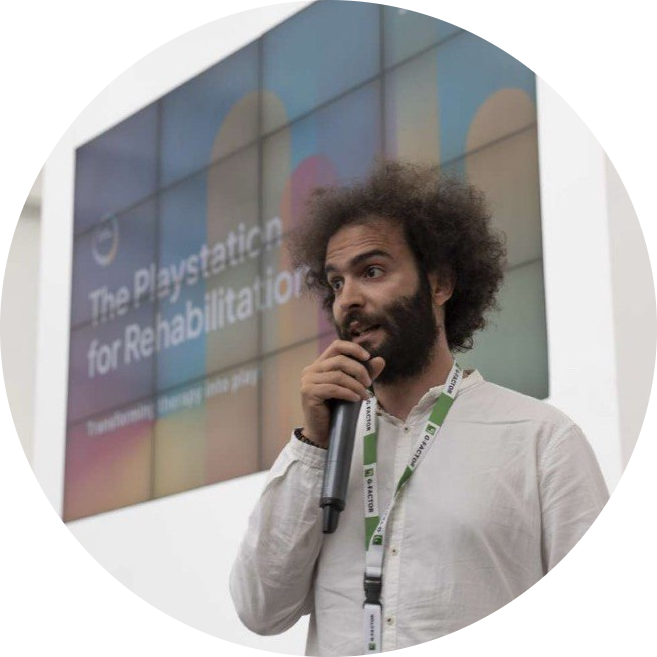
\includegraphics[width=2.8cm]{Pictures/Giovanni_pitch}
\end{minipage}
\vspace{0.1em}
}

\makeatletter
% the sender details are already in \clheader, so skip moderncv's own block
\@detailsfalse
% closing phrase, signature, name
\renewcommand*{\makeletterclosing}{%
  \@closing\\[0.6em]%
  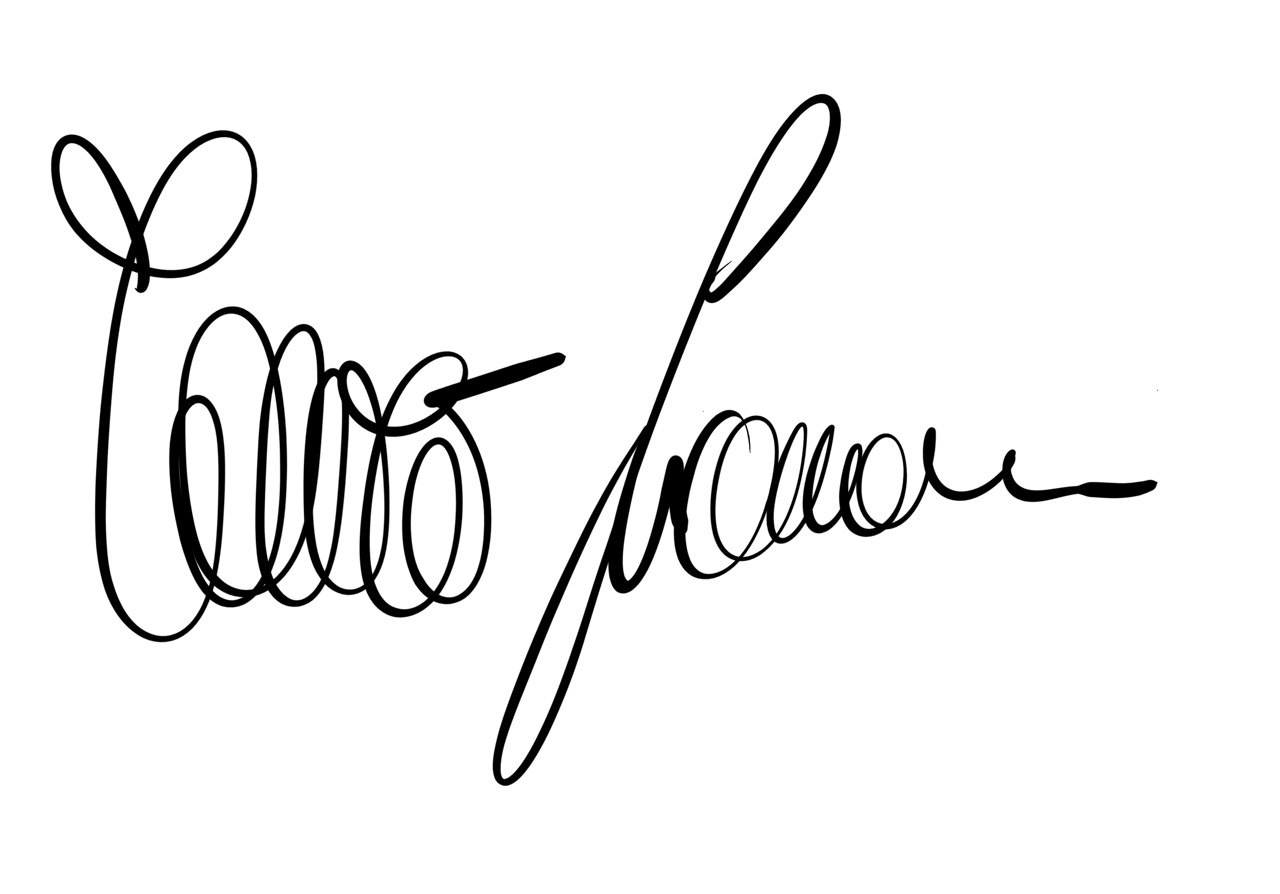
\includegraphics[height=1.2cm]{Pictures/sign_gt.jpg}\\[0.2em]%
  {\bfseries\@firstname~\@lastname}}
\makeatother


\begin{document}

\clheader{Experience Designer | UX for Complex, AI-enabled Systems}

\recipient{OCTO Hiring Team}{Pearson}
\opening{Dear Hiring Team,}
\closing{Yours faithfully,}
\makelettertitle

I am applying for the Lead Specialist, Experience Designer role (Req.\ 25428). I am a designer and engineer (MSc in Design \& Engineering, Politecnico di Milano) with more than five years making complex technical systems usable for the people who have to rely on them, at CNR-STIIMA, the Italian National Research Council, and as Head of Product and co-founder of Rehabilia Technologies.

The challenge you describe for Project Cookie, a front door that takes people from idea to deployment without exposing the machinery underneath, is the one I work on daily. I designed the interface of PhiCube, a rehabilitation device, together with Italian clinics, so that therapists could configure hardware and software without needing to understand them; it reached a usability score of 85.8/100 (SUS) with 19 children and is now in two multicentre studies with 134 patients.

I am at ease with dense, governed data. For my PhD project, OmniTrack, I designed and built OmniAnalytics, a web dashboard where researchers browse, compare and replay sessions. Much of the design went into the rules: flows to correct, exclude or relabel data while the raw records stay untouched, which is close to how an AI Inventory or a Semantic Layer must stay both open and trustworthy.

On AI, I co-authored research on socially interactive agents for robotic rehabilitation (Frontiers in Artificial Intelligence, 2024), I have built an embedded machine-learning classifier (TensorFlow Lite) into a prototype, and I prototype daily with Claude and Claude Code. I also code in React and Python, so I can test an idea with engineers early. Accessibility runs through my work, from OmniTrack, validated with 16 blind participants, to a game for children with cerebral palsy.

As Head of Product I own the process end to end and align engineering, clinical and business stakeholders on priorities and trade-offs. My work so far has been in healthcare and research rather than enterprise platforms; the problem of turning complexity into something people adopt and trust is the same. Examples are in the portfolio linked above.

I would welcome the chance to discuss the role further.

\makeletterclosing

\end{document}
